\documentclass{article}

\usepackage{amsmath}
\usepackage{graphicx}
\usepackage{subcaption}


\title{My first document}
\date{2021-10-27}
\author{Zion Umoh}

\begin{document}
	\section{Practice-1}
	Hello world!
	\pagenumbering{gobble}
	\maketitle
	\newpage
	\pagenumbering{arabic}
	Hello Class of 2021
	
	\section{Practice(4)-Section}
	Hello world!
	\subsection{Subsection}
	Structuring a document is easy
	\subsubsection{Subsubsection}
	More text
	\paragraph{Paragraph}
	Some more text
	\subparagraph{Subparagraph}
	Even more text
	\section{Another section}
	
	\section{Practice(5)Science Discoveries}
	Some of the \textbf{greatest}
	discoveries in \underline{Science}
	were made by
	\textbf{\textit{accident}}
	
	\paragraph{}
	Some of the greatest discoveries in science were made by \emph{accident}.
	
	\section{Practice-6}
		\begin{itemize}
		\item Ayomide
		\item Kamsi
		\item Eboseta
	\end{itemize}

\section{Practice-7}
\begin{enumerate}
	\item David
	\item Precious
	\item Tabitha
\end{enumerate}
\section{Practice-8}
	\begin{equation*}
	f(x)=x^2
\end{equation*}
\section{Practice-9}
	\begin{equation*}
	1 + 2 = 3
\end{equation*}
\begin{equation*}
	1 = 3 - 2
\end{equation*}
\begin{align*}
	1 + 2 &= 3\\
	1 &= 3 - 2
\end{align*}
\section{Practice-10}
	\begin{align*}
	f(x) &= x^2\\
	g(x) &= \frac{1}{x}\\
	F(x) &= \int^a_b
	\frac{1}{3}x^3
\end{align*}

\section{Practice-11}
	\begin{equation}
	\begin{matrix}
		1 & 0\\ 0 & 1
	\end{matrix}
\end{equation}
\section{Practice-12}
\begin{equation}
	[
	\begin{matrix}
		1 & 0\\
		0 & 1
	\end{matrix}
	]
\end{equation}
\section{Practice-13}
	\begin{equation*}
	\left[
	\begin{matrix}
		1 & 0\\
		0 & 1
	\end{matrix}
	\right]
\end{equation*}
\section{Practice-14}
	\begin{figure}
	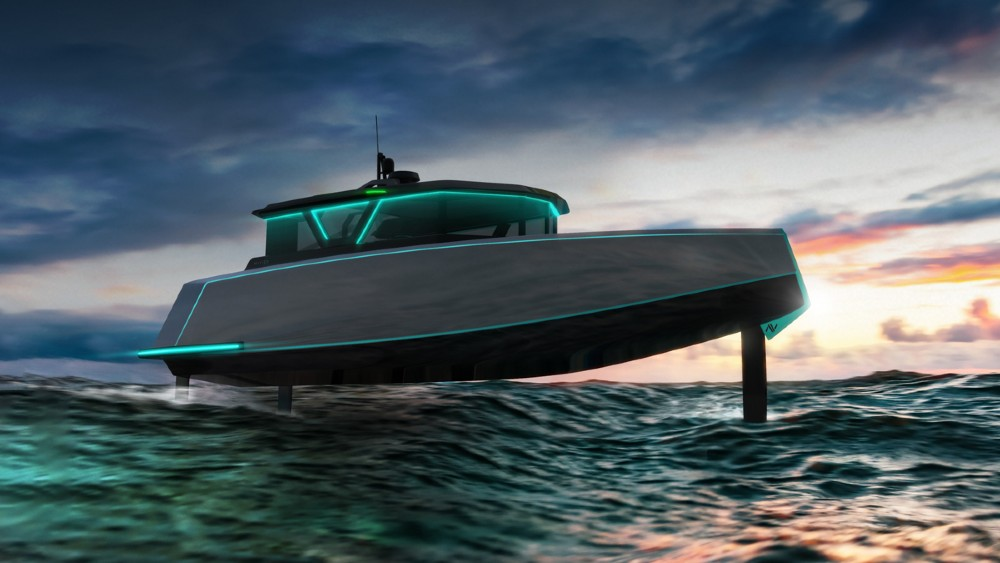
\includegraphics[width=\linewidth]{boat.jpg}
	\caption{A boat.}
	\label{fig:boat1}
\end{figure}
Figure \ref{fig:boat1} shows a boat 

\section{Practice-15}
	\begin{figure}[h!]
	\centering
	\begin{subfigure}[b]{0.4\linewidth}
		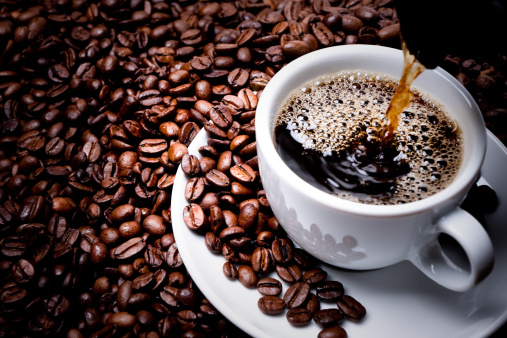
\includegraphics[width=\linewidth]{coffe.jpg}
		\caption{Coffee.}
	\end{subfigure}
	\begin{subfigure}[b]{0.4\linewidth}
		
		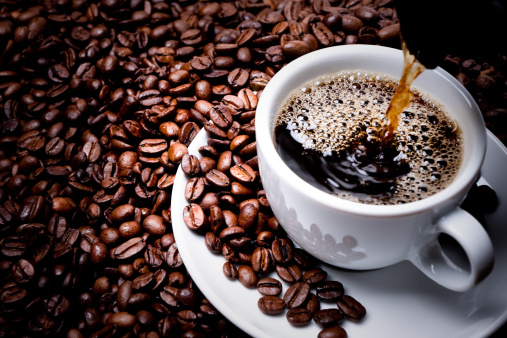
\includegraphics[width=\linewidth]{coffe.jpg}
		\caption{More coffee.}
	\end{subfigure}
	\caption{The same cup of coffee. Two times.}
	\label{fig:coffee}
\end{figure}

\section{Practice-16}
	\begin{figure}[h!]
	\centering
	\begin{subfigure}[b]{0.4\linewidth}
		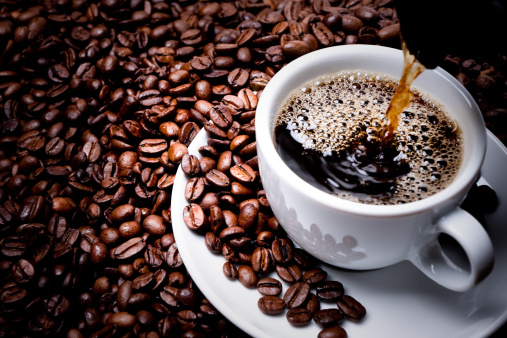
\includegraphics[width=\linewidth]{coffe.jpg}
		\caption{Coffee.}
	\end{subfigure}
	\begin{subfigure}[b]{0.4\linewidth}
		
		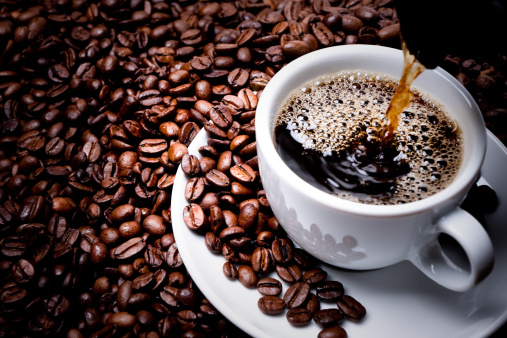
\includegraphics[width=\linewidth]{coffe.jpg}
		\caption{More coffee.}
	\end{subfigure}
	\caption{The same cup of coffee. Two times.}
	\label{fig:coffee}
\end{figure}
\end{document}